\section{Explaining the straddle account's profits}\label{sec:6}

The straddle signal forecasts persistent volatility richness. Its economic interpretation should also agree with the profits recorded by the backtester. We examine 2,599 executed straddle cohorts from January 2018 through 29 August 2025, retaining the learned sizing policy. This full-history attribution explains the straddle sleeve; it is separate from the later-period comparisons of learning policies.


\begin{figure}[!htbp]\centering
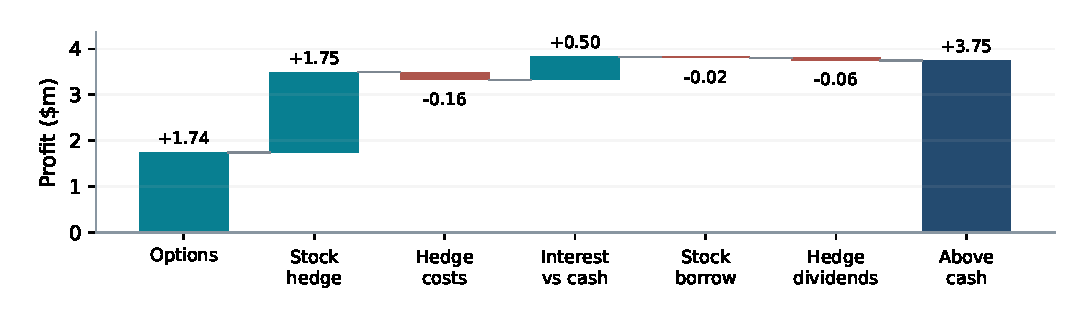
\includegraphics[width=\linewidth]{straddle_bridge.pdf}
\caption{Full-history straddle account, January 2018--August 2025. The option and stock components are read together; the remaining cash flows reconcile them to profit above cash.}\label{fig:straddle-bridge}
\end{figure}

Options after option charges earned \$1.74 million; stock hedges before hedge costs earned \$1.75 million. Together they earned \$3.49 million, reconciled to \$3.75 million above cash after the remaining costs, dividends and financing. Positive profits in both components do not establish two independent sources of alpha. Option marks contain time decay, price moves and volatility revaluation; the stock hedge is held to offset option delta.


\begin{figure}[!htbp]\centering
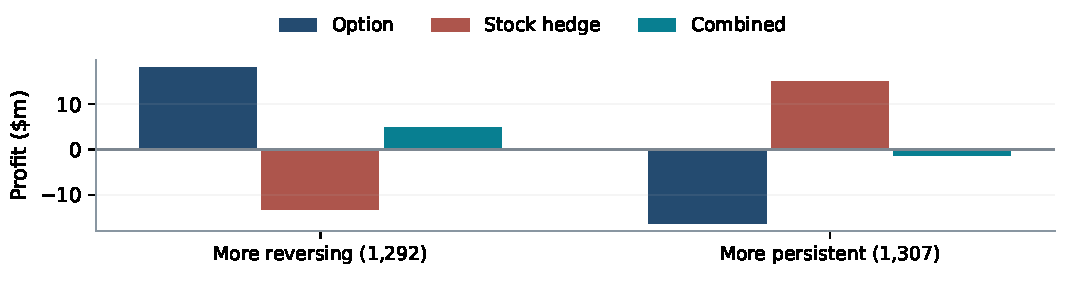
\includegraphics[width=\linewidth]{straddle_paths.pdf}
\caption{The same 2,599 cohorts grouped by their completed price paths. Combined profit includes option charges but precedes stock-hedge charges, dividends and financing. The grouping is descriptive.}\label{fig:straddle-paths}
\end{figure}

A short straddle has negative gamma. After a rising stock price, the delta hedge generally buys shares; after a fall, it sells. Continuing moves can reward the stock position while creating a larger option loss. Reversals can hurt the hedge while the option retains premium. In these cohorts, more reversing paths earn \$4.78 million together; more persistent paths lose \$1.29 million. The combined result is the relevant economic object.


Path persistence is the absolute entry-to-exit log return divided by the sum of absolute daily log returns. Values at or below 0.20 define the more reversing group. This grouping uses the completed path to explain results; it is not an available entry feature or a new trading rule.


\FloatBarrier
